\chapter{Thiết kế hệ thống}
\label{chap:system_design}

\section{Lập trình hướng đối tượng}
\label{sec:oop}
\textit{Lập trình hướng đối tượng} là phương pháp thiết kế phần mềm dựa trên các ``đối tượng'' mô tả dữ liệu và hành vi. Ở dự án WordSprint, mô‑đun backend được triển khai bằng C++20 và tuân thủ chặt chẽ các nguyên lý OOP:
\begin{itemize}
    \item Encapsulation (Đóng gói): Toàn bộ trạng thái phiên chơi gồm điểm số, chuỗi đúng liên tiếp (\code{currentStreak}), thời gian còn lại (\code{timeRemaining}) và danh sách câu hỏi được đóng gói bên trong lớp điều phối \code{GameSession}; lớp \code{User} đóng gói thông tin định danh và tùy chọn âm thanh cá nhân hóa qua phương thức \code{updateAudioPreferences}; lớp \code{Stage} đóng gói quy tắc đánh giá hoàn thành thông qua phương thức \code{isPassed(int score)}.
    \item Abstraction (Trừu tượng hóa): Lớp cơ sở trừu tượng \code{PuzzleQuestion} trừu tượng hóa các hành vi cốt lõi của một câu đố từ vựng thông qua các phương thức ảo thuần túy \code{generatePrompt()} và \code{checkAnswer(string input)}, đồng thời quản lý trạng thái hiển thị câu hỏi (\code{QuestionStatus}) và thực thể từ vựng (\code{WordItem}).
    \item Inheritance (Kế thừa): Ba dạng câu đố chuyên biệt gồm \code{ScrambleQuestion} (sắp xếp chữ cái), \code{FillBlankQuestion} (điền ký tự khuyết) và \code{AudioQuestion} (nghe phát âm đoán từ) kế thừa trực tiếp từ lớp trừu tượng \code{PuzzleQuestion}, tái sử dụng cấu trúc dùng chung và mở rộng các thuộc tính đặc thù.
    \item Polymorphism (Đa hình): Đối tượng điều phối \code{GameSession} tương tác với danh sách câu đố thông qua con trỏ hoặc tham chiếu tới lớp trừu tượng \code{PuzzleQuestion}. Khi gọi \code{generatePrompt()} hoặc \code{checkAnswer(input)}, cơ chế liên kết động (dynamic binding) tự động điều phối tới phương thức tương ứng của từng lớp câu đố cụ thể tại thời gian chạy.
\end{itemize}

\subsection{Biểu đồ lớp hướng đối tượng (Class Diagram)}
\label{subsec:class_diagram}

Kiến trúc các lớp đối tượng trong hệ thống WordSprint được mô hình hóa chi tiết trong Hình~\ref{fig:class_diagram}, thể hiện đầy đủ thuộc tính, phương thức và các mối quan hệ giữa các thực thể miền, bộ điều phối phiên chơi và phân cấp kế thừa câu đố.

\begin{figure}[!ht]
    \centering
    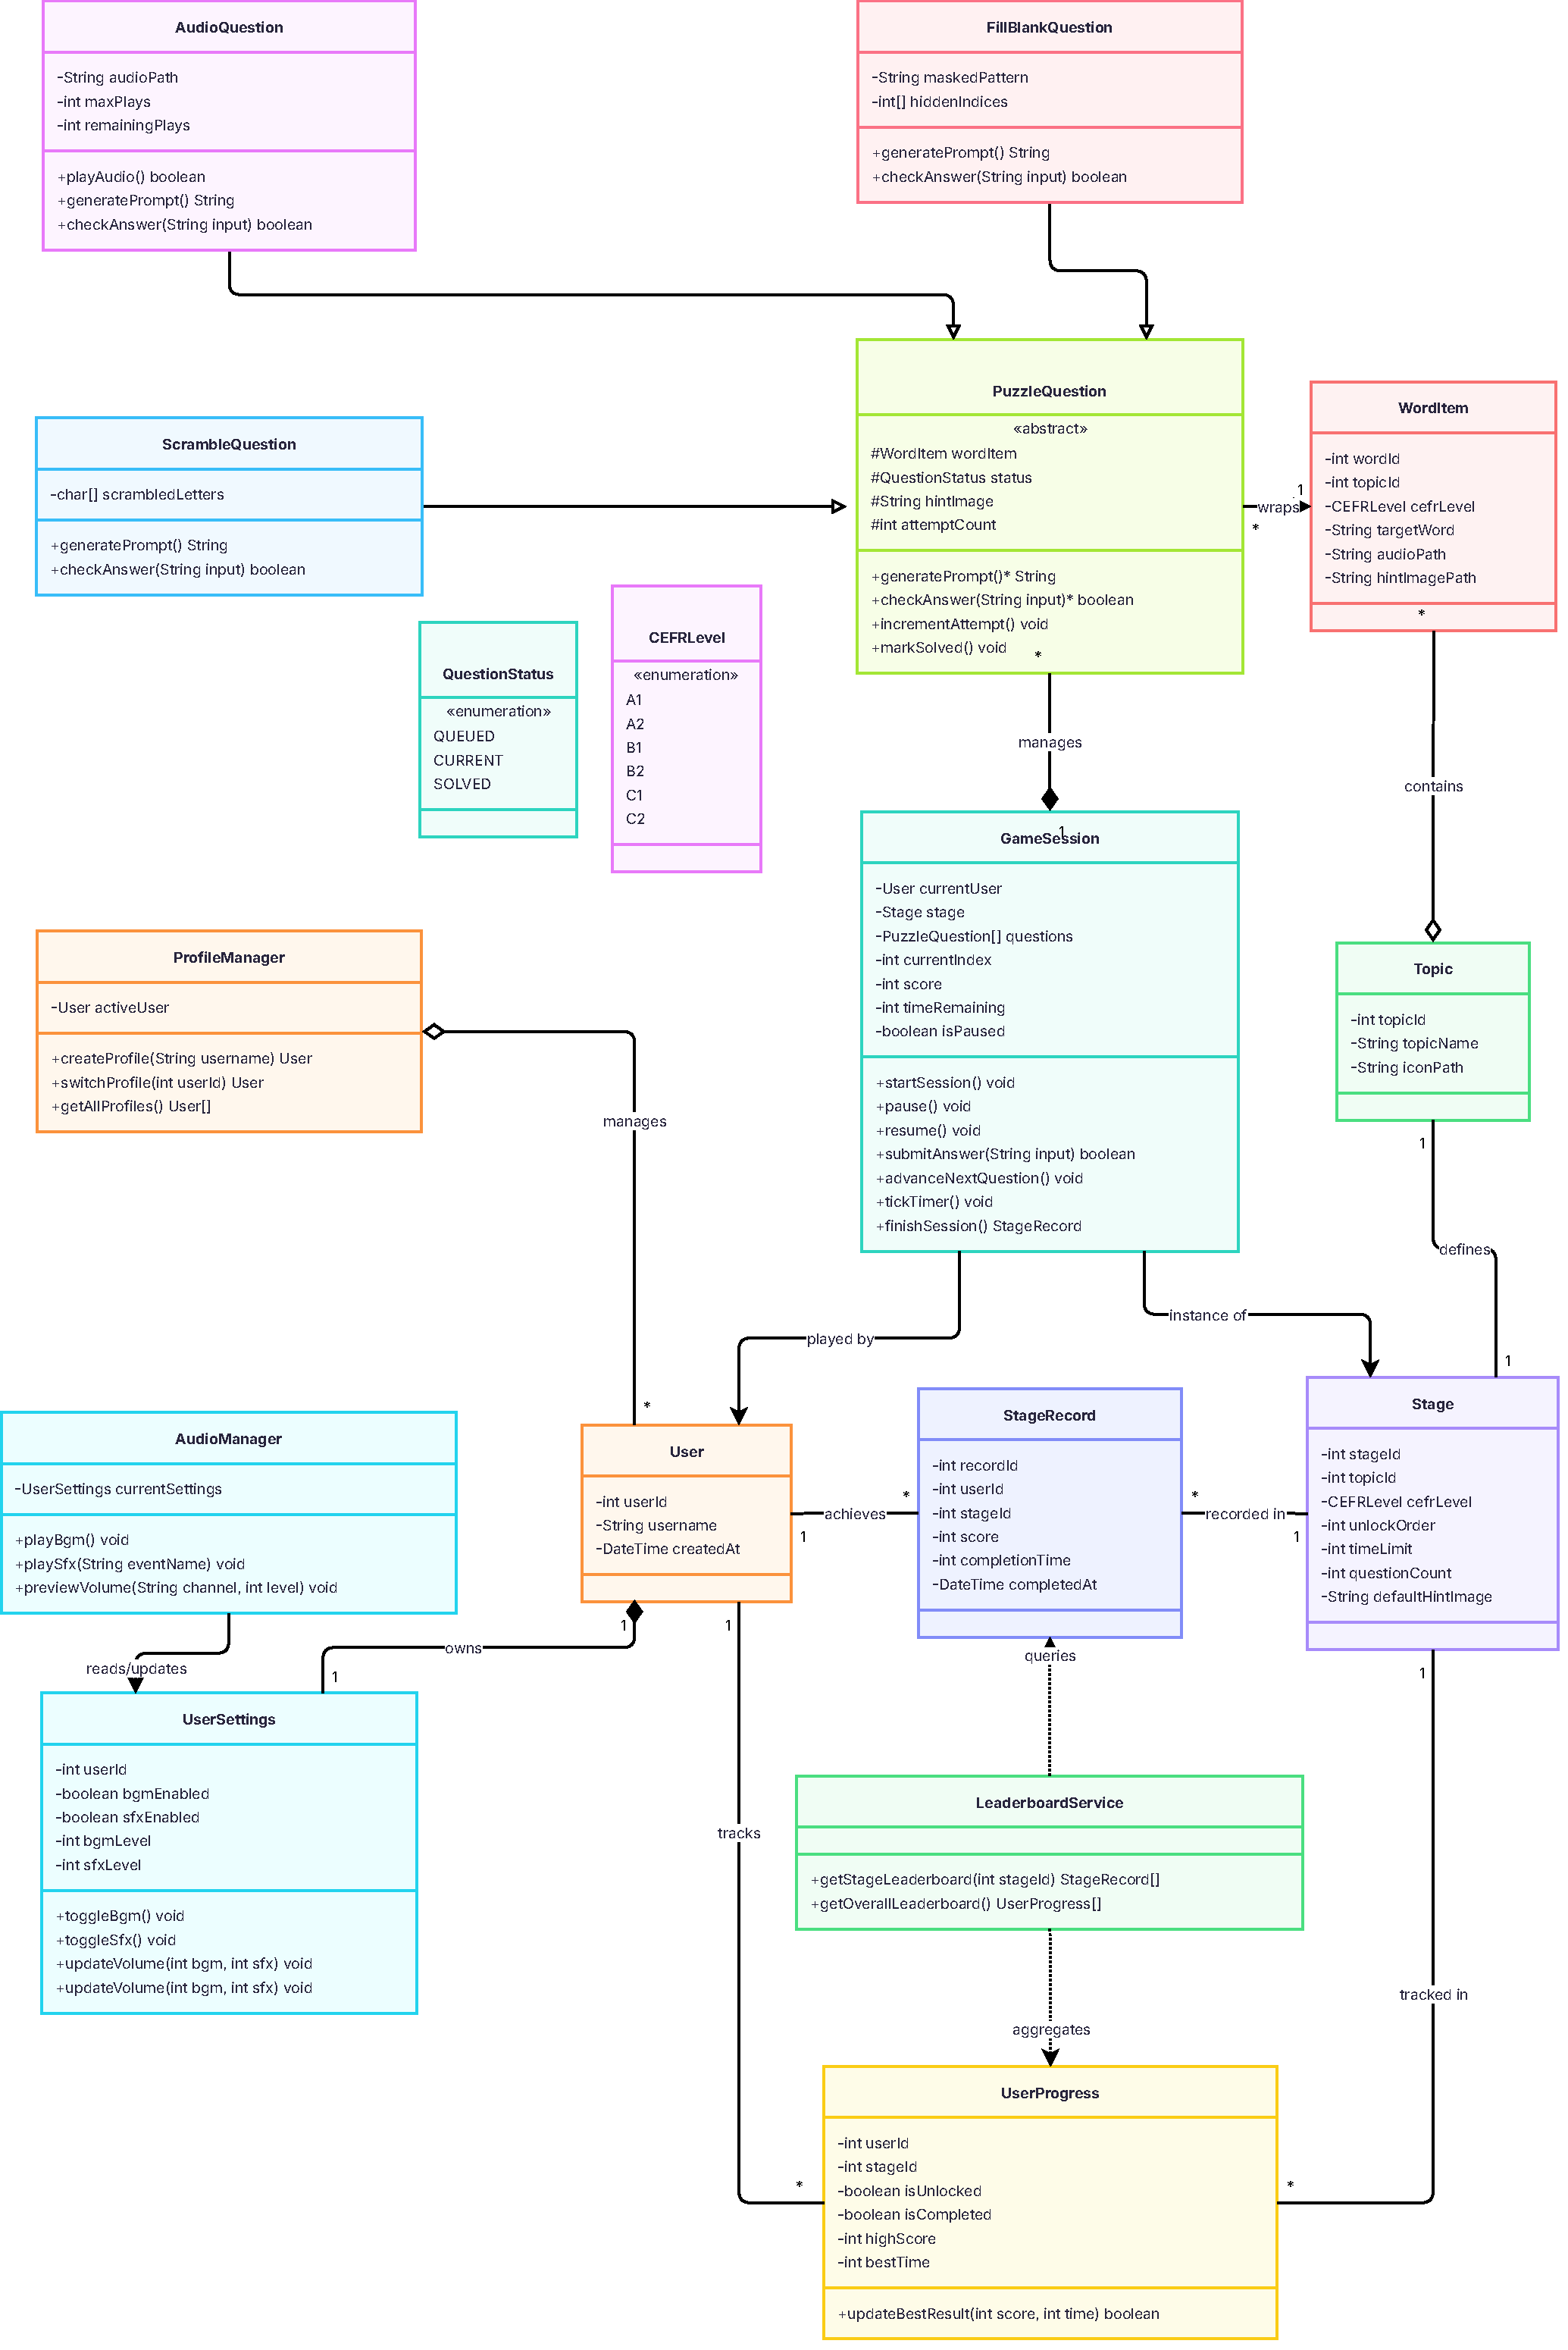
\includegraphics[max width=\linewidth, max height=0.75\textheight, keepaspectratio]{assets/figures/ch02/class_diagram.pdf}
    \caption{Biểu đồ lớp (Class Diagram) mô tả kiến trúc hướng đối tượng của WordSprint}
    \label{fig:class_diagram}
\end{figure}

Hệ thống lớp trong biểu đồ được phân thành bốn nhóm chính:
\begin{itemize}
    \item Nhóm điều phối phiên chơi: Trung tâm là lớp \code{GameSession}, chịu trách nhiệm quản lý vòng đời một lượt chơi, đếm thời gian (\code{tickTimer}), điều hướng câu hỏi (\code{advanceNextQuestion}), ghi nhận chuỗi thưởng và sinh bản ghi kết quả \code{StageRecord} khi kết thúc phiên (\code{finishSession}).
    \item Nhóm câu đố đa hình: Đứng đầu là lớp trừu tượng \code{PuzzleQuestion} liên kết 1--1 bao bọc \code{WordItem} và theo dõi trạng thái \code{QuestionStatus}. Ba lớp con \code{ScrambleQuestion}, \code{FillBlankQuestion} và \code{AudioQuestion} hiện thực hóa chi tiết thuật toán sinh đề và kiểm tra câu trả lời.
    \item Nhóm thực thể miền (Domain Entities): Bao gồm \code{User} (thông tin người chơi và tùy chỉnh âm thanh), \code{Topic} (chủ đề phân loại), \code{Stage} (cấu hình màn chơi kèm quy tắc đánh giá \code{isPassed}), \code{WordItem} (từ vựng kèm đường dẫn âm thanh và hình ảnh) và \code{StageRecord} (kết quả chi tiết của lượt chơi hoàn thành).
    \item Nhóm kiểu liệt kê (Enumerations): Bao gồm \code{CEFRLevel} (A1, A2, B1, B2, C1, C2) dùng để phân cấp độ khó của màn chơi và từ vựng; \code{QuestionStatus} (QUEUED, CURRENT, SOLVED) dùng để quản lý vòng đời hiển thị của từng câu đố trên giao diện.
\end{itemize}

\section{Ngôn ngữ C++ và CMake}
\label{sec:cpp_cmake}
Backend sử dụng C++20 để khai thác các tính năng hiện đại như \code{concepts}, \code{coroutines} (khi mở rộng), và \code{constexpr} để tối ưu hoá thời gian biên dịch.  Các tùy chọn biên dịch được định nghĩa trong \code{CMakeLists.txt}:
\begin{lstlisting}
cmake_minimum_required(VERSION 3.22)
project(WordSprint LANGUAGES CXX)
set(CMAKE_CXX_STANDARD 20)
set(CMAKE_CXX_STANDARD_REQUIRED ON)
add_subdirectory(backend)
\end{lstlisting}
CMake cung cấp khả năng phát hiện tự động vị trí Qt SDK (đường dẫn \code{C:/\allowbreak{}Qt/\allowbreak{}6.11.\allowbreak{}3/\allowbreak{}msvc2022\_\allowbreak{}64}) và tạo ra target \code{WordSprint} liên kết với \code{Qt6::Core}, \code{Qt6::Gui}, \code{Qt6::Qml}, \code{Qt6::WebEngineQuick}.

\section{Giao diện người dùng}
\label{sec:frontend}
Phần giao diện được xây dựng bằng React 19 và công cụ xây dựng nhanh Vite.  Kiến trúc dự án frontend tuân thủ mô hình component‑based, mỗi màn hình trò chơi được biểu diễn bằng một component React độc lập (\code{Game.jsx}, \code{ScoreBoard.jsx}).  Tailwind CSS 4 được tích hợp để tạo kiểu nhanh chóng, hỗ trợ thiết kế \textit{neo‑brutalism} với màu sắc và đường viền mạnh mẽ.

\section{Cơ chế giao tiếp giữa backend và frontend}
\label{sec:communication}
Qt WebEngineView được sử dụng để nhúng ứng dụng web React vào ứng dụng desktop Qt. Ứng dụng khởi tạo một \code{QUrl} tới URL Vite dev server (\code{http:\allowbreak{}//\allowbreak{}localhost:\allowbreak{}5173}) hoặc tới file tĩnh \code{index.html} đã được build. Trong \code{main.cpp}:
Frontend và backend trao đổi dữ liệu thông qua WebChannel (\code{QtWebChannel}) – các đối tượng C++ được đăng ký vào context, cho phép JavaScript gọi các phương thức C++.

\section{Thiết kế tương tác với biểu đồ tuần tự}
\label{sec:interaction_design}

Để làm rõ trình tự trao đổi thông điệp theo trục thời gian giữa tác nhân người chơi, đối tượng điều phối phiên chơi và các kho dữ liệu, hệ thống được mô hình hóa thông qua hai biểu đồ tuần tự đại diện cho hai luồng tương tác quan trọng nhất trong một phiên giải đố: khởi tạo phiên chơi và gửi câu trả lời kèm hoàn thành màn.

\subsection{Biểu đồ tuần tự luồng bắt đầu màn chơi}
\label{subsec:seq_start_stage}

Biểu đồ tuần tự trong Hình~\ref{fig:seq_start_stage} mô tả quy trình khởi tạo phiên chơi khi người chơi chọn một màn chơi hợp lệ từ bản đồ chủ đề và cấp độ CEFR. Toàn bộ quá trình chuẩn bị dữ liệu và sinh câu đố diễn ra tuần tự qua các bước:

\begin{enumerate}
    \item Người chơi (Player) gửi thông điệp \code{startSession(user, stage)} tới đối tượng điều phối phiên chơi \code{GameSession}.
    \item Đối tượng \code{GameSession} gọi phương thức \code{getRandomWords(stage.topicId, stage.cefrLevel, stage.questionCount)} trên kho dữ liệu \code{StageRepository} để truy vấn danh sách từ vựng ngẫu nhiên khớp với chủ đề và cấp độ CEFR đã chọn.
    \item Kho dữ liệu \code{StageRepository} thực thi truy vấn SQLite và trả về danh sách các thực thể từ vựng \code{wordList : WordItem[]}.
    \item Đối tượng \code{GameSession} thực hiện giải thuật nội bộ \code{assignShuffledQuizTypes(wordList)} để phân phối ngẫu nhiên cân bằng ba dạng câu đố (Scramble, Fill-in-the-Blank, Audio) vào túi bài tập (bag).
    \item Vòng lặp \code{loop [For each (wordItem, quizType) in bag]} duyệt qua từng phần tử để sinh tập câu đố:
    \begin{itemize}
        \item Khởi tạo đối tượng câu đố đa hình cụ thể thông qua thông điệp \code{<<create>> create(wordItem, quizType, stage.cefrLevel)} gửi tới hệ thống phân cấp \code{PuzzleQuestion}.
        \item \code{GameSession} gọi phương thức ảo \code{generatePrompt()} trên đối tượng câu đố vừa khởi tạo để nhận về dữ liệu gợi ý và đề bài \code{promptData}.
    \end{itemize}
    \item Cuối cùng, \code{GameSession} gọi phương thức nội bộ \code{initState(score = 0, streak = 0, timeRemaining = stage.timeLimit)} để thiết lập trạng thái ban đầu, kích hoạt đồng hồ đếm ngược và bắt đầu phiên chơi.
\end{enumerate}

\begin{figure}[!ht]
    \centering
    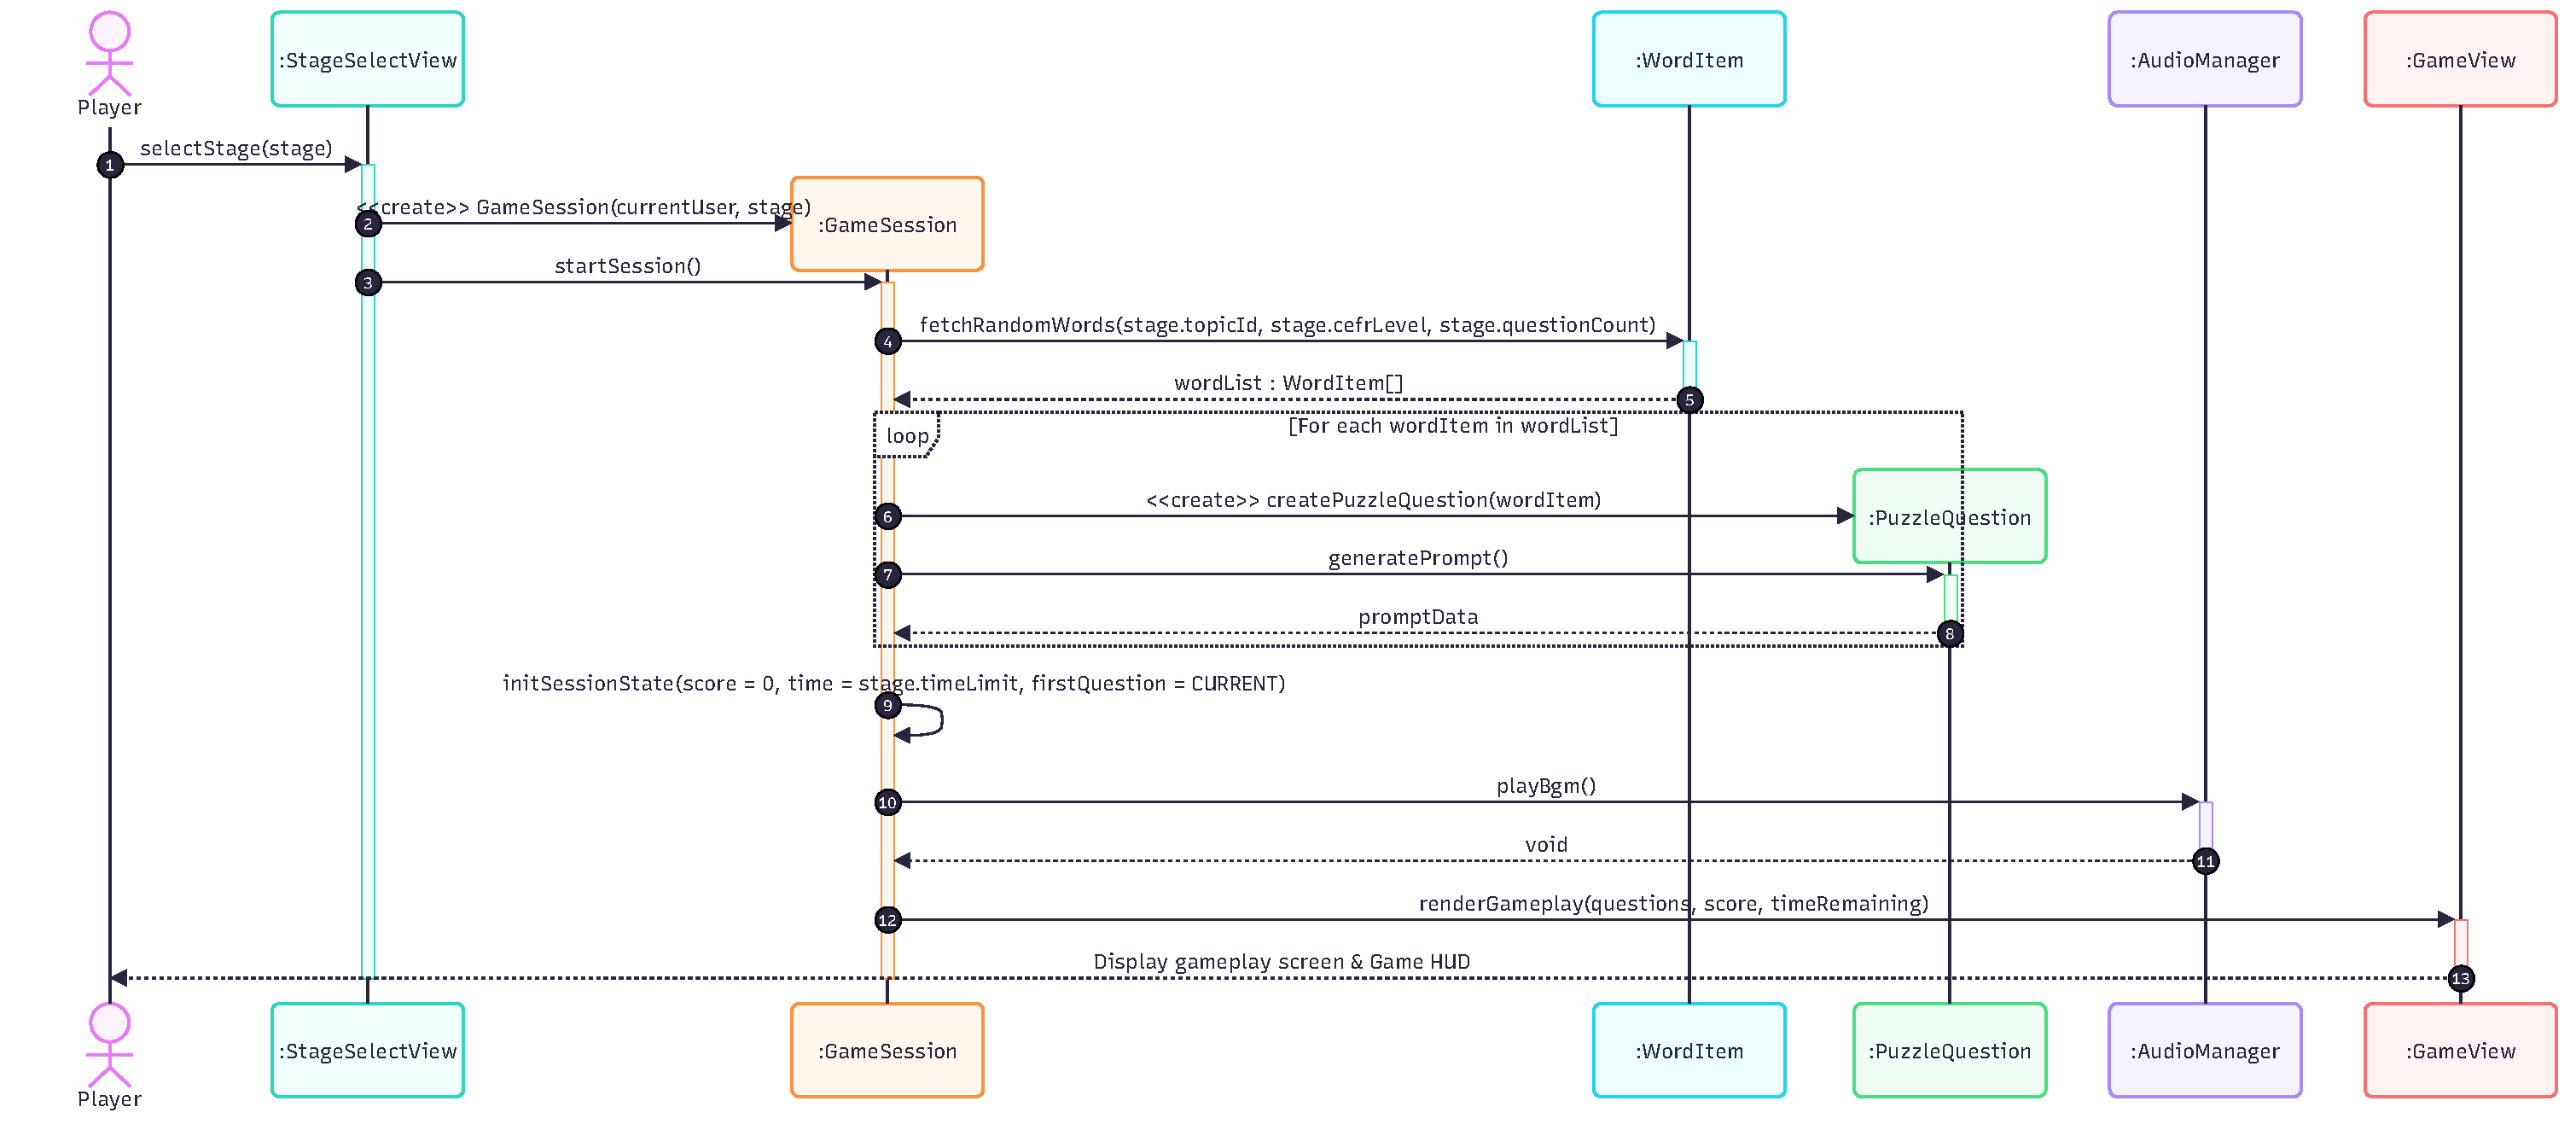
\includegraphics[max width=\linewidth, max height=0.75\textheight, keepaspectratio]{assets/figures/ch02/sequence_diagram_start_stage.pdf}
    \caption{Biểu đồ tuần tự luồng bắt đầu màn chơi}
    \label{fig:seq_start_stage}
\end{figure}

\subsection{Biểu đồ tuần tự luồng xác nhận đáp án và hoàn thành màn chơi}
\label{subsec:seq_complete_stage}

Biểu đồ tuần tự trong Hình~\ref{fig:seq_complete_stage} mô tả quy trình tiếp nhận câu trả lời, tính điểm chuỗi liên tiếp và lưu trữ kết quả khi hoàn thành toàn bộ câu hỏi của màn chơi:

\begin{enumerate}
    \item Người chơi (Player) nhập từ vựng và gửi thông điệp \code{submitAnswer(input)} tới đối tượng điều phối \code{GameSession}.
    \item Đối tượng \code{GameSession} chuyển tiếp yêu cầu kiểm tra tới câu đố hiện tại thông qua phương thức đa hình \code{checkAnswer(input)} trên \code{PuzzleQuestion}.
    \item Câu đố đối chiếu đáp án với từ gốc \code{targetWord} và trả về kết quả \code{isCorrect : boolean}.
    \item Trong trường hợp trả lời sai (\code{alt [isCorrect == false]}): \code{GameSession} gọi phương thức nội bộ \code{resetStreak()} để đưa biến đếm chuỗi đúng liên tiếp về 0.
    \item Trong trường hợp trả lời đúng (\code{alt [isCorrect == true]}):
    \begin{itemize}
        \item \code{GameSession} gọi phương thức \code{markSolved()} trên \code{PuzzleQuestion} để đánh dấu câu đố chuyển sang trạng thái \code{SOLVED}.
        \item \code{GameSession} gọi phương thức nội bộ \code{incrementStreak()} để tăng chuỗi câu trả lời đúng liên tiếp.
        \item \code{GameSession} gọi phương thức nội bộ \code{addScore(stage.cefrLevel, currentStreak)} để tính điểm cơ bản kèm điểm thưởng chuỗi cộng dồn vào tổng điểm phiên chơi.
        \item Nhánh rẽ tiếp theo:
        \begin{itemize}
            \item Nếu vẫn còn câu hỏi chưa giải (\code{alt [Unsolved questions remain]}): \code{GameSession} gọi \code{advanceNextQuestion()} để chuyển quyền điều khiển sang câu hỏi tiếp theo trong danh sách.
            \item Nếu toàn bộ câu hỏi đã được giải đúng (\code{alt [All questions solved]}):
            \begin{enumerate}
                \item \code{GameSession} gọi \code{finishSession()} để dừng đồng hồ đếm ngược và tổng hợp thời gian hoàn thành thực tế.
                \item Khởi tạo thực thể bản ghi kết quả \code{<<create>> StageRecord(user.userId, stage.stageId, score, completionTime)}.
                \item Gửi thông điệp \code{save(record)} tới kho dữ liệu \code{RecordRepository} để lưu trữ bản ghi vào bảng \code{stage\_records} và nhận về đối tượng \code{savedRecord : StageRecord}.
                \item \code{GameSession} gọi phương thức \code{isPassed(score)} trên thực thể \code{Stage} để đối chiếu điểm đạt được với ngưỡng chuẩn \code{passScore} và nhận về kết quả boolean xác nhận việc hoàn thành vượt màn.
            \end{enumerate}
        \end{itemize}
    \end{itemize}
\end{enumerate}

\begin{figure}[!ht]
    \centering
    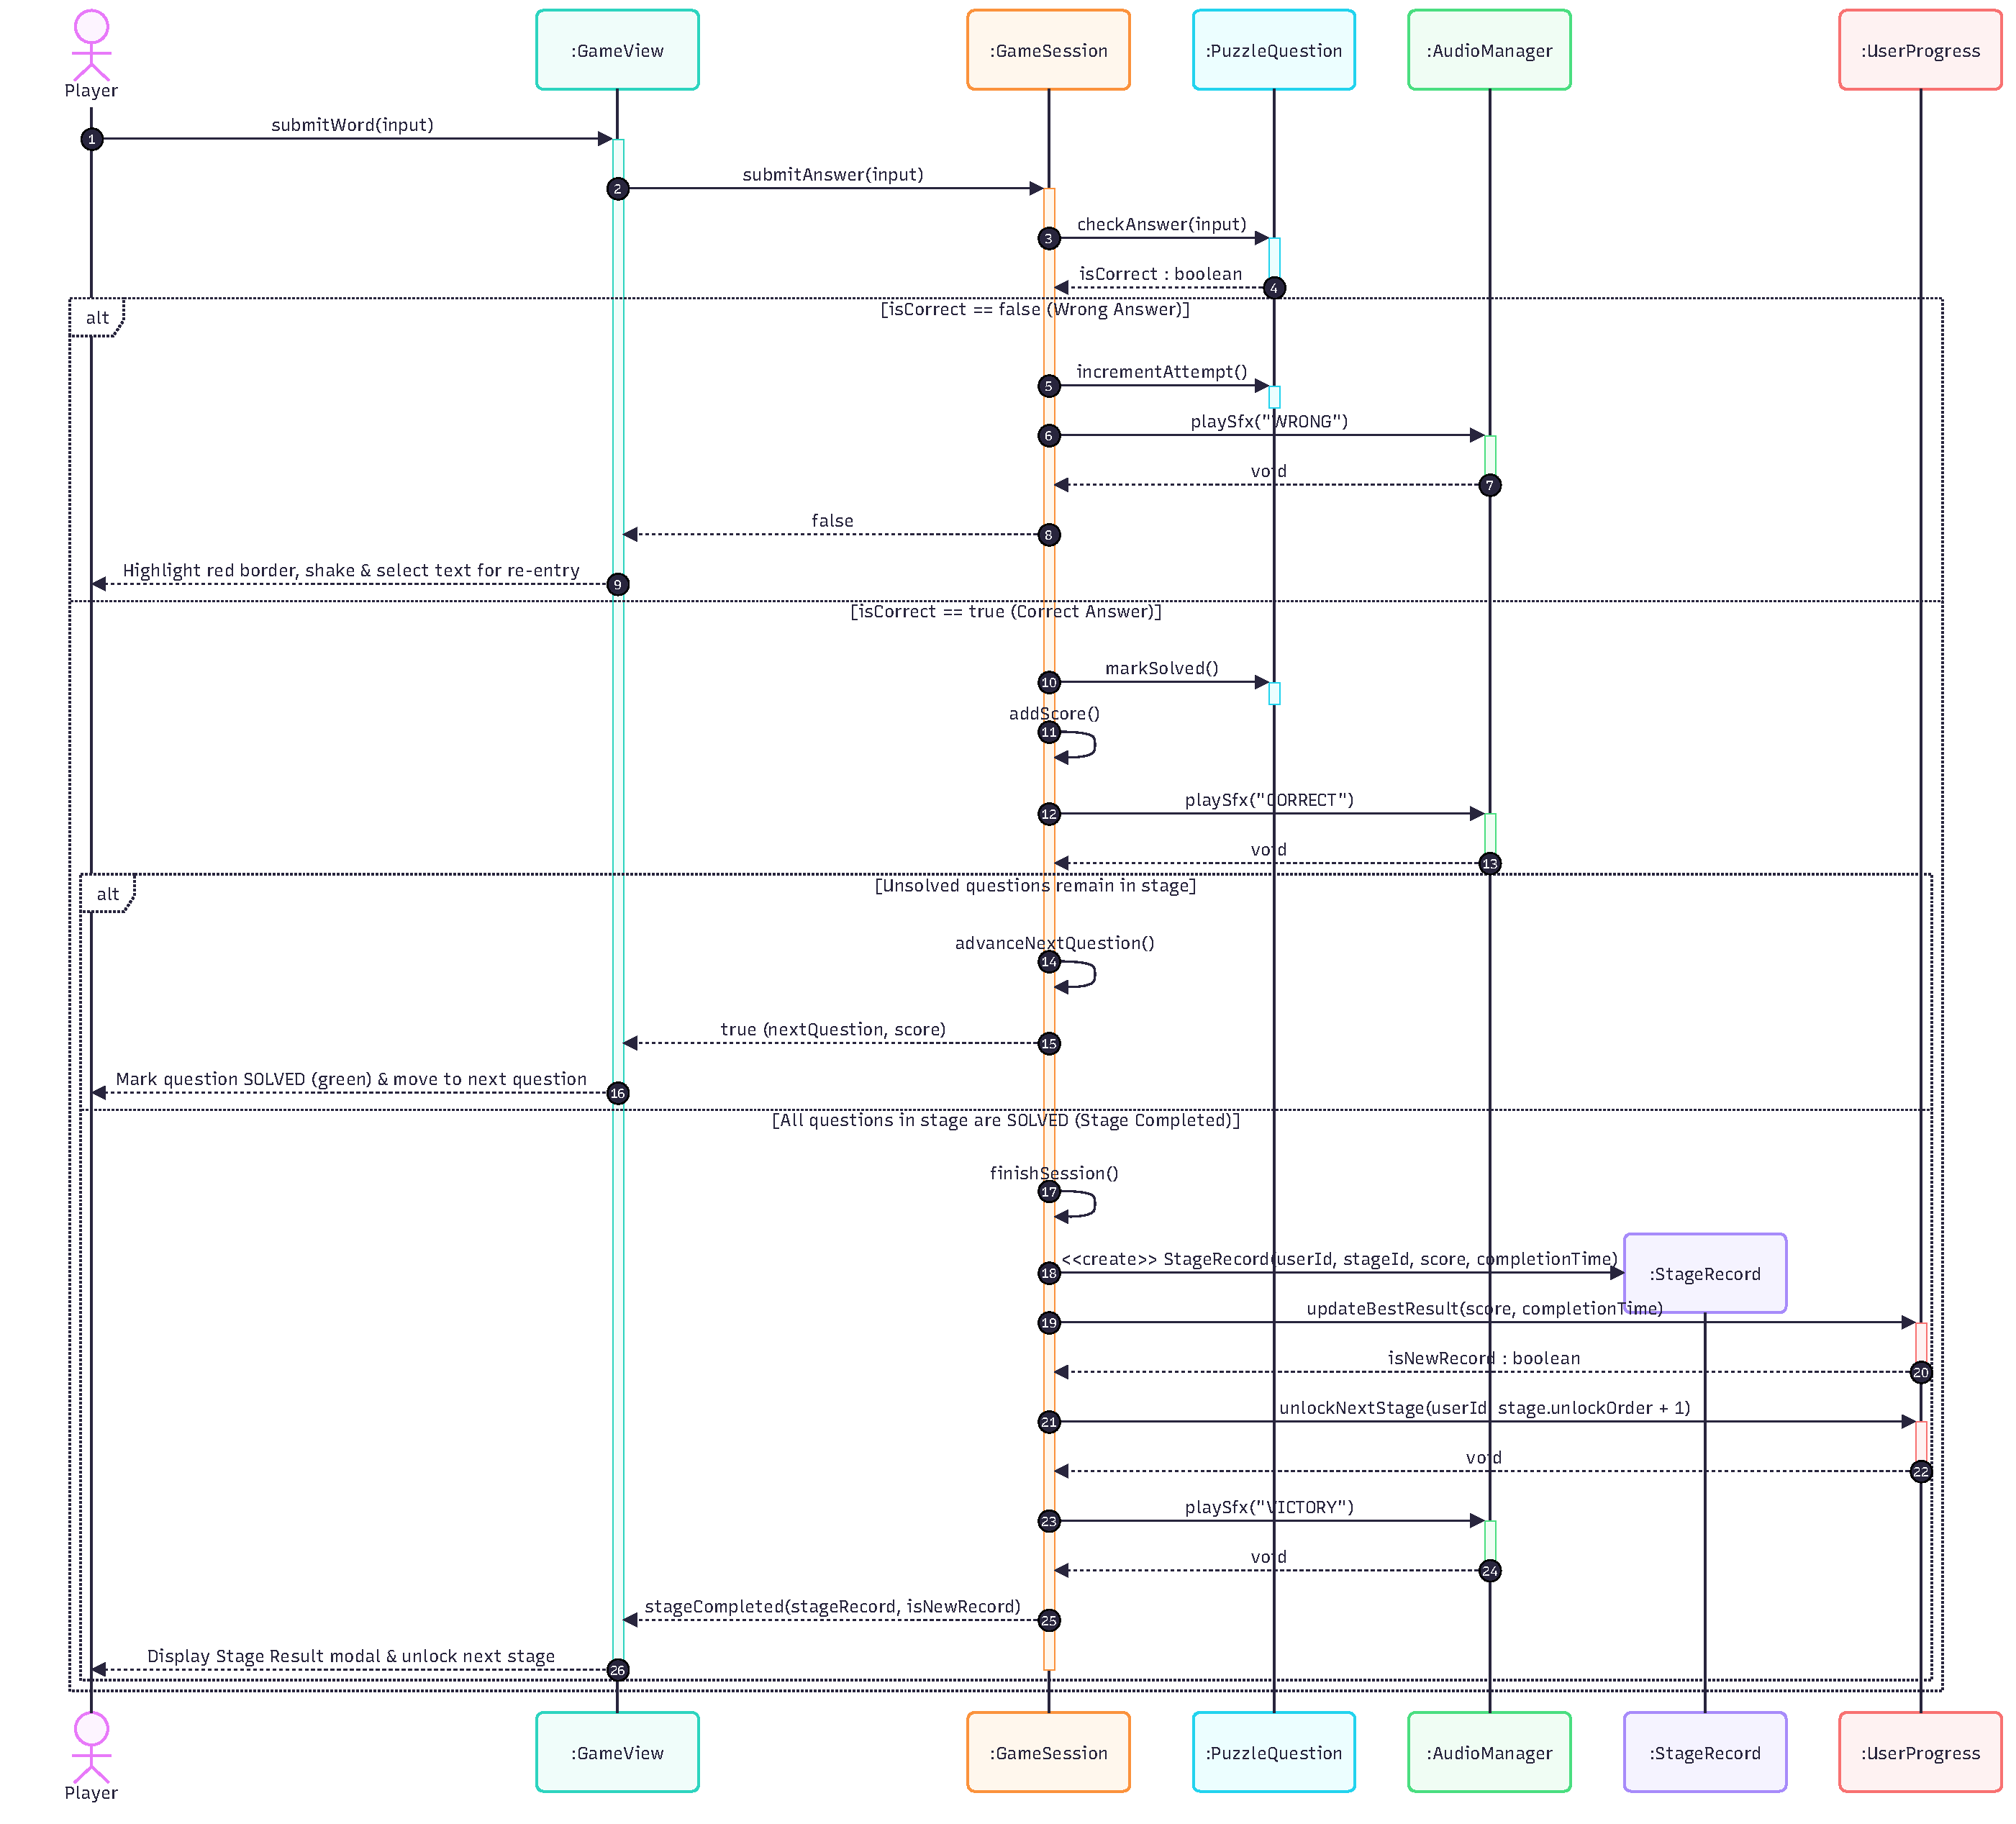
\includegraphics[max width=\linewidth, max height=0.75\textheight, keepaspectratio]{assets/figures/ch02/sequence_diagram_submit_puzzle_answer.pdf}
    \caption{Biểu đồ tuần tự luồng xác nhận đáp án và hoàn thành màn chơi}
    \label{fig:seq_complete_stage}
\end{figure}
\FloatBarrier

\section{Thiết kế cơ sở dữ liệu}
\label{sec:database_design}

Hệ thống sử dụng hệ quản trị cơ sở dữ liệu quan hệ nhúng SQLite nhằm lưu trữ toàn bộ dữ liệu bền vững ngay trên máy tính cá nhân của người dùng. Cơ sở dữ liệu gồm năm bảng quan hệ, được kích hoạt cơ chế kiểm tra toàn vẹn khóa ngoại ngay khi khởi tạo kết nối để đảm bảo tính nhất quán tuyệt đối giữa các hồ sơ người chơi, cấu hình âm thanh, kho từ vựng và lịch sử lượt chơi.

\subsection{Mô hình thực thể kết hợp và quan hệ giữa các bảng}
\label{subsec:erd}

Các thực thể trong cơ sở dữ liệu được tổ chức tinh gọn theo nguyên tắc nguồn dữ liệu duy nhất (Single Source of Truth), phục vụ đồng thời hai nhóm nghiệp vụ chính là lưu trữ kho học liệu từ vựng và quản lý dữ liệu cá nhân hóa của từng người chơi:

\begin{itemize}
    \item Bảng \code{users}: Lưu trữ thông tin định danh của từng người chơi và tích hợp trực tiếp các cấu hình âm thanh cá nhân hóa gồm trạng thái bật/tắt (\code{bgm\_enabled}, \code{sfx\_enabled}) và mức âm lượng (\code{bgm\_volume}, \code{sfx\_volume}). Việc tích hợp các trường này giúp đọc nhanh toàn bộ hồ sơ trong một truy vấn duy nhất mà không cần tạo bảng phụ một--một.
    \item Bảng \code{topics} và quan hệ một‑nhiều với \code{stages} và \code{word\_pool}: Bảng \code{topics} tinh giản chỉ gồm mã định danh \code{topic\_id} và tên chủ đề \code{topic\_name}. Một chủ đề phân loại nhiều màn chơi theo các cấp độ CEFR khác nhau (thông qua ràng buộc duy nhất phức hợp giữa mã chủ đề và cấp độ CEFR) và quản lý kho từ vựng dùng chung cho các màn thuộc chủ đề đó.
    \item Bảng \code{stages}: Định nghĩa cấu hình chi tiết cho từng màn chơi, gồm cấp độ \code{cefr\_level}, thời gian đếm ngược \code{time\_limit}, số lượng câu hỏi \code{question\_count} và điểm số tối thiểu để vượt màn \code{pass\_score}. Ràng buộc duy nhất phức hợp trên cặp \code{(topic\_id, cefr\_level)} đảm bảo mỗi chủ đề chỉ tồn tại duy nhất một màn chơi cho mỗi cấp độ CEFR.
    \item Bảng \code{word\_pool}: Lưu trữ các mục từ vựng tiếng Anh theo từng chủ đề và cấp độ khó, gồm từ gốc \code{target\_word}, đường dẫn âm thanh \code{audio\_path} và hình ảnh minh họa \code{hint\_image\_path}. Các hình thức câu đố (xáo trộn hoặc điền khuyết) được sinh tự động tại thời gian chạy từ từ gốc, không cần lưu trữ chuỗi gợi ý tĩnh.
    \item Bảng \code{stage\_records} và quan hệ nhiều‑nhiều giữa \code{users} và \code{stages}: Đóng vai trò là nguồn dữ liệu duy nhất ghi lại toàn bộ lịch sử các lượt chơi hoàn thành. Mỗi bản ghi lưu giữ điểm số \code{score}, thời gian thực tế \code{completion\_time} và thời điểm chơi \code{played\_at}. Mọi thông tin về kỷ lục cá nhân, tiến độ mở khóa cấp độ CEFR và thứ hạng bảng xếp hạng đều được truy vấn trực tiếp từ bảng này.
\end{itemize}

Để tối ưu hóa tốc độ truy xuất khi kho từ vựng mở rộng hoặc khi người chơi mở bảng xếp hạng, cơ sở dữ liệu thiết lập các chỉ mục tìm kiếm quan trọng:

\begin{itemize}
    \item Chỉ mục phức hợp trên bảng \code{word\_pool} gồm hai cột \code{topic\_id} và \code{cefr\_level} giúp lọc nhanh danh sách từ vựng ứng viên trước khi chọn ngẫu nhiên bộ câu hỏi lúc bắt đầu màn chơi.
    \item Chỉ mục phức hợp trên bảng \code{stage\_records} gồm các cột \code{stage\_id}, \code{score} (sắp xếp giảm dần) và \code{completion\_time} (sắp xếp tăng dần) giúp truy vấn tức thì danh sách kỷ lục dẫn đầu ở từng màn chơi (Per-Stage Top 10).
    \item Chỉ mục trên cột \code{user\_id} của bảng \code{stage\_records} giúp tổng hợp nhanh tiến độ vượt cấp độ CEFR và điểm số tích lũy của từng người chơi.
\end{itemize}

\begin{figure}[!ht]
    \centering
    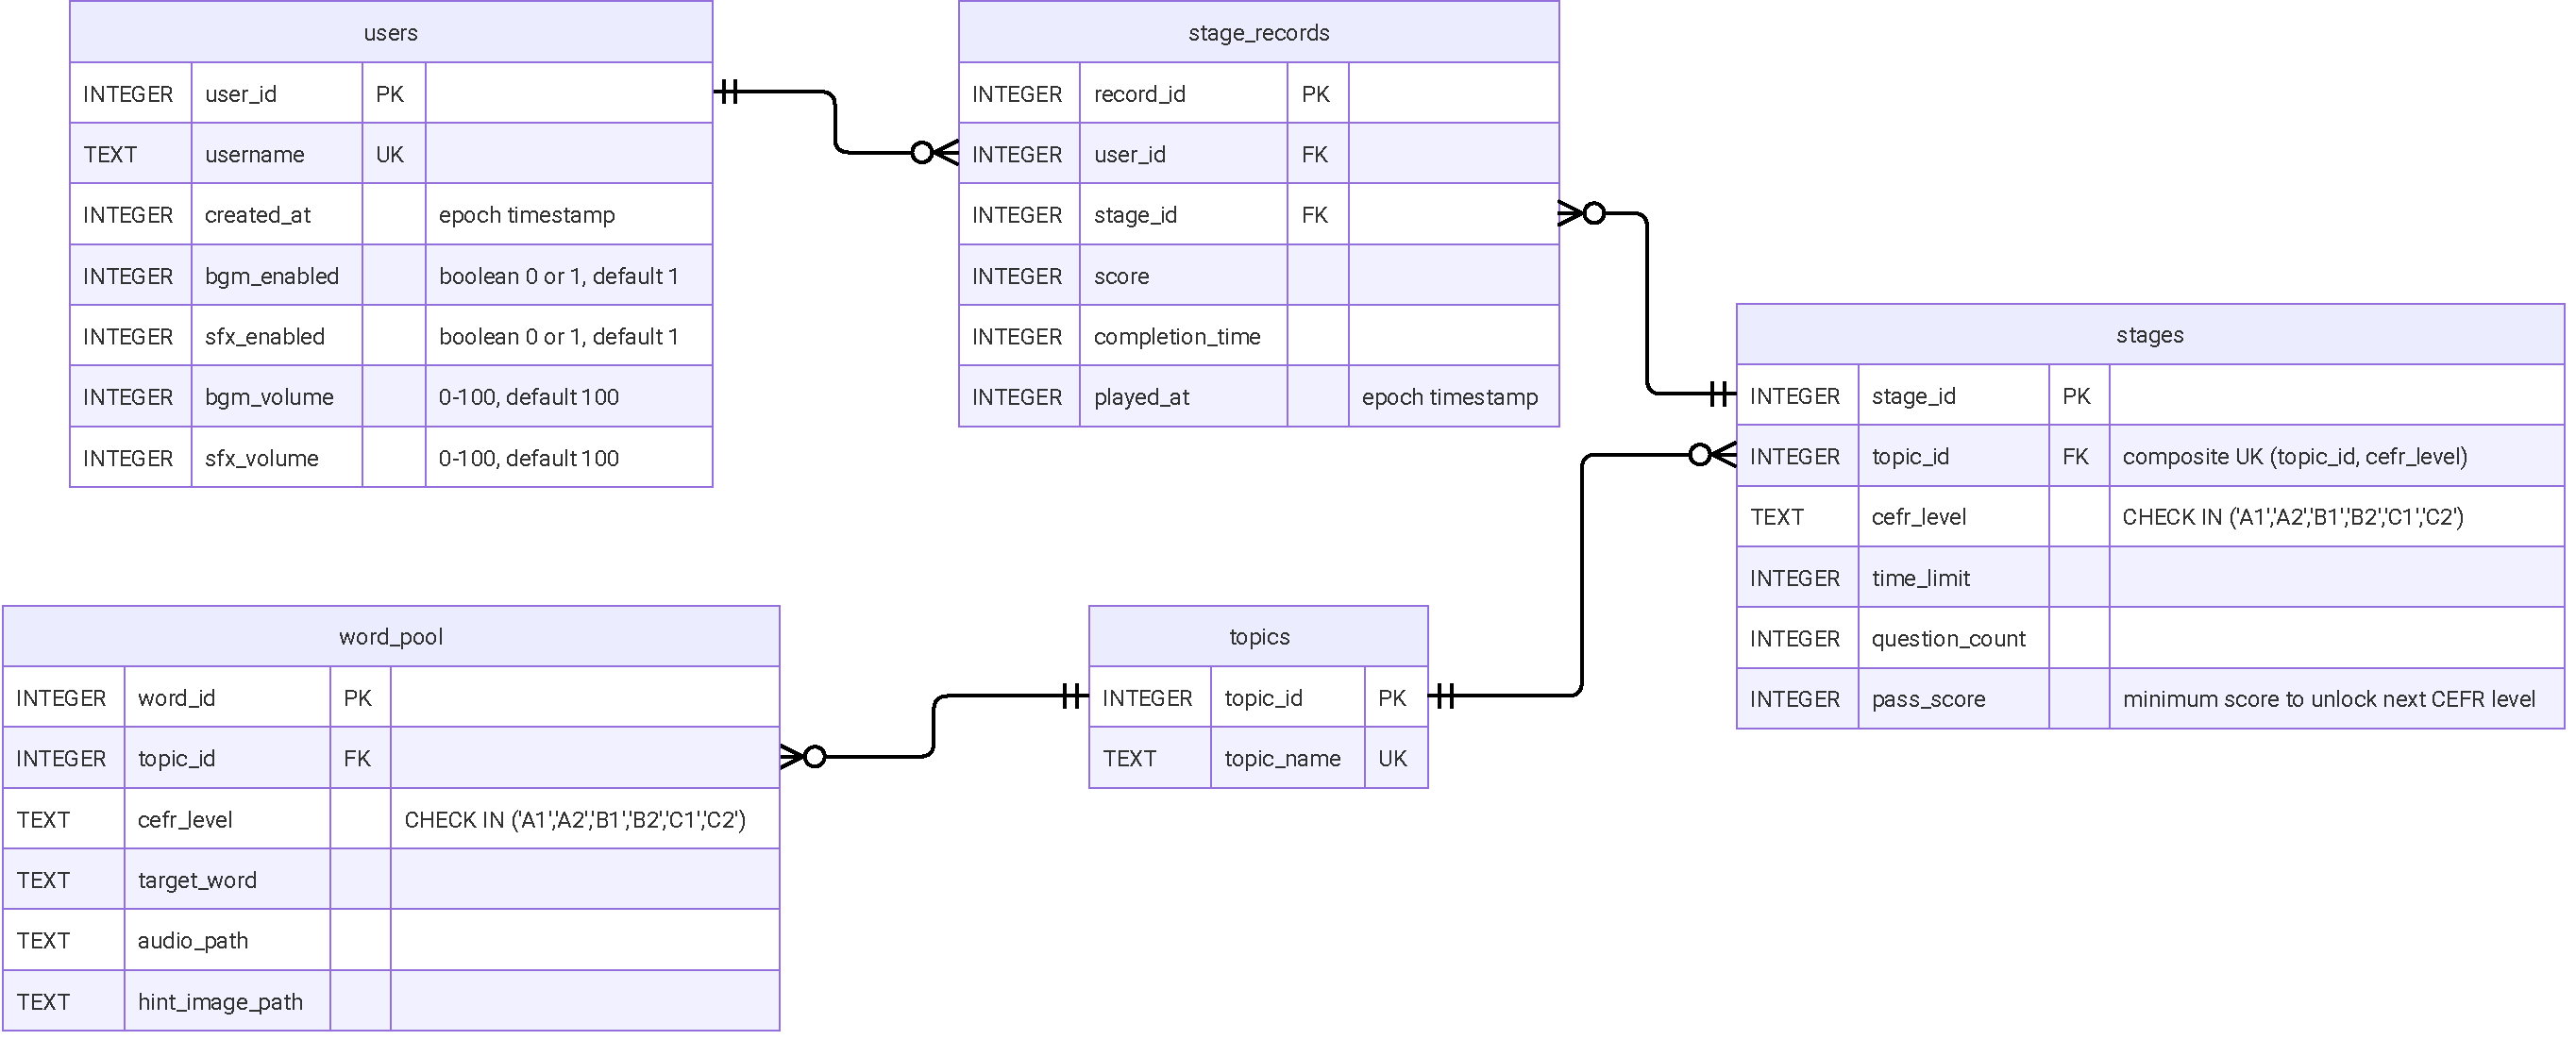
\includegraphics[max width=\linewidth, max height=0.75\textheight, keepaspectratio]{assets/figures/ch02/entity_relationship_diagram.pdf}
    \caption{Biểu đồ thực thể kết hợp (ERD) của cơ sở dữ liệu WordSprint}
    \label{fig:erd}
\end{figure}

\subsection{Đặc tả cấu trúc các bảng}
\label{subsec:table_specs}

\begin{xltabular}{\textwidth}{|N|N|Y|Y|}
\caption{Đặc tả cấu trúc bảng users}
\label{tab:users}
\\
\hline
\thcell{Tên cột} & \thcell{Kiểu dữ liệu} & \thcell{Khóa và ràng buộc} & \thcell{Mô tả} \\
\hline
\endfirsthead
\hline
\thcell{Tên cột} & \thcell{Kiểu dữ liệu} & \thcell{Khóa và ràng buộc} & \thcell{Mô tả} \\
\hline
\endhead
user\_id & INTEGER & Khóa chính, tự động tăng & Mã định danh duy nhất của hồ sơ người chơi \\
\hline
username & TEXT & Duy nhất, không rỗng & Tên hiển thị của người chơi dùng để phân biệt các hồ sơ \\
\hline
created\_at & INTEGER & Không rỗng, thời gian khởi tạo & Dấu thời gian (epoch timestamp) khởi tạo hồ sơ trên thiết bị \\
\hline
bgm\_enabled & INTEGER & Không rỗng, mặc định 1 & Trạng thái bật nhạc nền (1 là bật, 0 là tắt) \\
\hline
sfx\_enabled & INTEGER & Không rỗng, mặc định 1 & Trạng thái bật hiệu ứng âm thanh (1 là bật, 0 là tắt) \\
\hline
bgm\_volume & INTEGER & Không rỗng, mặc định 100 & Mức âm lượng nhạc nền (từ 0 đến 100) \\
\hline
sfx\_volume & INTEGER & Không rỗng, mặc định 100 & Mức âm lượng hiệu ứng âm thanh (từ 0 đến 100) \\
\hline
\end{xltabular}

\begin{xltabular}{\textwidth}{|N|N|Y|Y|}
\caption{Đặc tả cấu trúc bảng topics}
\label{tab:topics}
\\
\hline
\thcell{Tên cột} & \thcell{Kiểu dữ liệu} & \thcell{Khóa và ràng buộc} & \thcell{Mô tả} \\
\hline
\endfirsthead
\hline
\thcell{Tên cột} & \thcell{Kiểu dữ liệu} & \thcell{Khóa và ràng buộc} & \thcell{Mô tả} \\
\hline
\endhead
topic\_id & INTEGER & Khóa chính, tự động tăng & Mã định danh duy nhất của chủ đề từ vựng \\
\hline
topic\_name & TEXT & Duy nhất, không rỗng & Tên chủ đề (ví dụ: Daily Communication, Travel, IT) \\
\hline
\end{xltabular}

\begin{xltabular}{\textwidth}{|N|N|Y|Y|}
\caption{Đặc tả cấu trúc bảng stages}
\label{tab:stages}
\\
\hline
\thcell{Tên cột} & \thcell{Kiểu dữ liệu} & \thcell{Khóa và ràng buộc} & \thcell{Mô tả} \\
\hline
\endfirsthead
\hline
\thcell{Tên cột} & \thcell{Kiểu dữ liệu} & \thcell{Khóa và ràng buộc} & \thcell{Mô tả} \\
\hline
\endhead
stage\_id & INTEGER & Khóa chính, tự động tăng & Mã định danh duy nhất của màn chơi \\
\hline
topic\_id & INTEGER & Không rỗng, khóa ngoại \code{topics(\allowbreak topic\_id)} & Mã chủ đề trực thuộc (khóa duy nhất phức hợp cùng \code{cefr\_level}) \\
\hline
cefr\_level & TEXT & Không rỗng, A1--C2 & Cấp độ từ vựng chuẩn CEFR áp dụng cho màn chơi \\
\hline
time\_limit & INTEGER & Không rỗng, thời gian quy định & Giới hạn thời gian đếm ngược của màn chơi (giây) \\
\hline
question\_count & INTEGER & Không rỗng, số lượng câu & Số lượng câu hỏi cần giải trong một lượt chơi \\
\hline
pass\_score & INTEGER & Không rỗng, điểm chuẩn tối thiểu & Điểm số tối thiểu cần đạt để vượt màn và mở khóa cấp độ CEFR tiếp theo \\
\hline
\end{xltabular}

\begin{xltabular}{\textwidth}{|N|N|Y|Y|}
\caption{Đặc tả cấu trúc bảng word\_pool}
\label{tab:word_pool}
\\
\hline
\thcell{Tên cột} & \thcell{Kiểu dữ liệu} & \thcell{Khóa và ràng buộc} & \thcell{Mô tả} \\
\hline
\endfirsthead
\hline
\thcell{Tên cột} & \thcell{Kiểu dữ liệu} & \thcell{Khóa và ràng buộc} & \thcell{Mô tả} \\
\hline
\endhead
word\_id & INTEGER & Khóa chính, tự động tăng & Mã định danh duy nhất của mục từ vựng \\
\hline
topic\_id & INTEGER & Không rỗng, khóa ngoại \code{topics(\allowbreak topic\_id)} & Mã chủ đề phân loại từ vựng \\
\hline
cefr\_level & TEXT & Không rỗng, A1--C2 & Cấp độ khó của từ vựng theo chuẩn CEFR \\
\hline
target\_word & TEXT & Không rỗng & Từ vựng tiếng Anh gốc dùng làm đáp án câu đố \\
\hline
audio\_path & TEXT & Đường dẫn tệp & Đường dẫn tới tệp âm thanh phát âm chuẩn \\
\hline
hint\_image\_path & TEXT & Cho phép rỗng & Đường dẫn tới hình ảnh minh họa gợi ý \\
\hline
\end{xltabular}

\begin{xltabular}{\textwidth}{|N|N|Y|Y|}
\caption{Đặc tả cấu trúc bảng stage\_records}
\label{tab:stage_records}
\\
\hline
\thcell{Tên cột} & \thcell{Kiểu dữ liệu} & \thcell{Khóa và ràng buộc} & \thcell{Mô tả} \\
\hline
\endfirsthead
\hline
\thcell{Tên cột} & \thcell{Kiểu dữ liệu} & \thcell{Khóa và ràng buộc} & \thcell{Mô tả} \\
\hline
\endhead
record\_id & INTEGER & Khóa chính, tự động tăng & Mã định danh duy nhất của bản ghi lịch sử lượt chơi \\
\hline
user\_id & INTEGER & Không rỗng, khóa ngoại \code{users(\allowbreak user\_id)} & Mã hồ sơ người chơi thực hiện lượt chơi \\
\hline
stage\_id & INTEGER & Không rỗng, khóa ngoại \code{stages(\allowbreak stage\_id)} & Mã màn chơi tương ứng với lượt chơi \\
\hline
score & INTEGER & Không rỗng & Tổng điểm số đạt được trong lượt chơi \\
\hline
completion\_time & INTEGER & Không rỗng & Tổng thời gian thực tế (giây) hoàn thành toàn bộ câu hỏi \\
\hline
played\_at & INTEGER & Không rỗng, thời gian kết thúc & Dấu thời gian (epoch timestamp) hoàn thành lượt chơi \\
\hline
\end{xltabular}

\section{Thiết kế cơ chế trò chơi và giải thuật tính toán}
\label{sec:game_mechanisms}

Để đảm bảo trò chơi vừa mang tính giáo dục vừa kích thích sự hứng thú lâu dài của người học, hệ thống WordSprint xây dựng bộ quy tắc cơ chế trò chơi (Game Mechanism) dựa trên mô hình cơ sở dữ liệu 5 bảng tinh giản, chuẩn hóa từ cấp độ khó, nhịp độ thử thách, thuật toán sinh câu đố đến hệ thống tính điểm và bảng xếp hạng.

\subsection{Vòng lặp trải nghiệm và cơ chế mở khóa theo cấp độ CEFR}
\label{subsec:gameplay_loop_and_progression}

Vòng lặp trải nghiệm cốt lõi của trò chơi được vận hành khép kín qua 5 bước chính:
\begin{enumerate}
    \item Chọn hồ sơ người chơi: Người chơi đăng nhập hoặc chọn hồ sơ cá nhân; hệ thống nạp toàn bộ tùy chọn âm thanh (\code{bgm\_enabled}, \code{sfx\_enabled}, \code{bgm\_volume}, \code{sfx\_volume}) và tổng hợp tiến độ hiện tại từ \code{stage\_records}.
    \item Chọn cấp độ và chủ đề: Người chơi lựa chọn cấp độ CEFR đã mở khóa (từ A1 đến C2) và chọn chủ đề từ vựng mong muốn.
    \item Thực hiện phiên giải đố: Hệ thống truy vấn ngẫu nhiên \code{question\_count} từ vựng từ \code{word\_pool} khớp với cặp \code{(topic\_id, cefr\_level)}, sau đó tự động xáo trộn và phân bổ đều giữa ba hình thức (Scramble, Fill-in-the-Blank, Audio) trong giới hạn thời gian \code{time\_limit}.
    \item Ghi nhận kết quả lượt chơi: Khi hoàn thành câu hỏi cuối cùng hoặc hết giờ đếm ngược, thông số lượt chơi được ghi nhận nguyên tử vào \code{stage\_records}.
    \item Mở khóa cấp độ và cập nhật xếp hạng: Nếu $\text{score} \ge \text{pass\_score}$, hệ thống tự động mở khóa toàn bộ các chủ đề ở cấp độ CEFR kế tiếp, đồng thời cập nhật vị trí xếp hạng của người chơi.
\end{enumerate}

Khác với mô hình mở khóa tuần tự cứng nhắc, WordSprint áp dụng cơ chế \textit{Mở khóa theo cấp độ CEFR} (Tier-based Unlock):
\begin{itemize}
    \item Người chơi mới luôn được mở khóa sẵn toàn bộ các chủ đề ở cấp độ A1.
    \item Chỉ cần hoàn thành đạt chuẩn ($\text{score} \ge \text{pass\_score}$) tại bất kỳ một chủ đề nào ở cấp độ $N$, toàn bộ các chủ đề ở cấp độ kế tiếp $N+1$ sẽ đồng loạt được mở khóa.
    \item Người chơi có toàn quyền chơi lại bất kỳ màn chơi nào đã mở khóa để phá kỷ lục điểm số cá nhân hoặc nâng cao thứ hạng trên bảng xếp hạng Top 10.
\end{itemize}

\subsection{Phân cấp cấu trúc màn chơi và giới hạn thời gian}
\label{subsec:stage_structure_and_pacing}

Nhằm tạo ra thử thách phù hợp với từng giai đoạn phát triển trình độ tiếng Anh, các tham số màn chơi được hiệu chỉnh tăng tiến theo từng bậc CEFR như trình bày trong Bảng~\ref{tab:stage_structure}.

\begin{xltabular}{\textwidth}{|N|N|N|N|Y|}
\caption{Cấu trúc thông số màn chơi theo từng bậc chuẩn CEFR}
\label{tab:stage_structure}
\\
\hline
\thcell{Cấp độ CEFR} & \thcell{Số câu hỏi} & \thcell{Thời gian (s)} & \thcell{Điểm gốc / từ} & \thcell{Điểm chuẩn (\code{pass\_score})} \\
\hline
\endfirsthead
\hline
\thcell{Cấp độ CEFR} & \thcell{Số câu hỏi} & \thcell{Thời gian (s)} & \thcell{Điểm gốc / từ} & \thcell{Điểm chuẩn (\code{pass\_score})} \\
\hline
\endhead
A1 (Cơ bản) & 10 & 90 (1p 30s) & 10 & 70 (đạt 7/10 câu = 70\%) \\
\hline
A2 (Sơ cấp) & 10 & 100 (1p 40s) & 15 & 105 (đạt 7/10 câu = 70\%) \\
\hline
B1 (Trung cấp) & 12 & 120 (2p 00s) & 20 & 160 (đạt 8/12 câu $\approx$ 67\%) \\
\hline
B2 (Trung cao cấp) & 12 & 135 (2p 15s) & 25 & 225 (đạt 9/12 câu = 75\%) \\
\hline
C1 (Cao cấp) & 15 & 165 (2p 45s) & 30 & 330 (đạt 11/15 câu $\approx$ 73\%) \\
\hline
C2 (Thành thạo) & 15 & 180 (3p 00s) & 35 & 385 (đạt 11/15 câu $\approx$ 73\%) \\
\hline
\end{xltabular}

Đồng hồ đếm ngược hoạt động liên tục từ \code{time\_limit} về 0. Khi người chơi giải đúng câu hỏi cuối cùng, đồng hồ được dừng lập tức và ghi nhận thời gian thực tế:
\begin{equation}
\label{eq:completion_time}
\text{completion\_time} = \text{time\_limit} - \text{remaining\_time}
\end{equation}

\subsection{Giải thuật sinh câu đố thích ứng}
\label{subsec:puzzle_algorithms}

Hệ thống kết hợp kỹ thuật xáo trộn phân phối đều (Bag Randomization) để cân bằng ba dạng câu đố trong mỗi màn:
\begin{itemize}
    \item Dạng Sắp xếp chữ cái (Scramble): Các chữ cái trong \code{target\_word} được xáo trộn ngẫu nhiên liên tục cho đến khi chuỗi kết quả khác chuỗi gốc. Đối với các cụm từ gồm nhiều từ đơn, giải thuật bảo toàn vị trí khoảng trắng và chỉ xáo trộn nội bộ trong từng từ. Hình ảnh minh họa (\code{hint\_image\_path}) được hiển thị hỗ trợ suy luận.
    \item Dạng Điền khuyết (Fill-in-the-Blank): Số lượng ký tự bị ẩn được tính toán tự động dựa trên độ dài từ và cấp độ CEFR thông qua công thức:
    \begin{equation}
    \label{eq:hidden_count}
    \text{hidden\_count} = \operatorname{clamp}\left(\operatorname{round}(L \times r),\, 1,\, L - 1\right)
    \end{equation}
    trong đó $L$ là tổng số ký tự chữ cái của từ, $r$ là tỷ lệ ẩn tương ứng với độ khó: $r = 0{,}35$ cho A1--A2 (trong đó chữ cái đầu tiên luôn được giữ cố định), $r = 0{,}50$ cho B1--B2 và $r = 0{,}65$ cho C1--C2.
    \item Dạng Nghe âm thanh (Audio): Chỉ áp dụng cho từ có tệp âm thanh hợp lệ (\code{audio\_path} khác rỗng). Hệ thống tự động phát âm một lần khi tải câu hỏi và hỗ trợ người chơi nghe lại thủ công với số lượt giới hạn: $3$ lần cho A1--A2, $2$ lần cho B1--B2 và $1$ lần cho C1--C2. Hình ảnh gợi ý được ẩn hoàn toàn để đảm bảo đánh giá đúng kỹ năng nghe.
\end{itemize}

\subsection{Hệ thống tính điểm và chuỗi liên tiếp (Streak Bonus)}
\label{subsec:scoring_and_streak}

Để khuyến khích sự tập trung và độ chính xác liên tục, điểm số thưởng chuỗi được áp dụng từ câu trả lời đúng thứ ba trở đi. Gọi $B$ là điểm số cơ bản cho mỗi câu đúng tương ứng với cấp độ CEFR ($B \in \{10, 15, 20, 25, 30, 35\}$) và $k$ là số câu trả lời đúng liên tiếp hiện tại ($k = 1, 2, 3, \dots$):

\begin{equation}
\label{eq:score}
\text{Points Earned} = \begin{cases}
B, & \text{khi } 1 \le k \le 2 \\
B + 2, & \text{khi } k \ge 3
\end{cases}
\end{equation}

Mỗi khi người chơi trả lời sai hoặc chọn bỏ qua câu hỏi, biến đếm chuỗi lập tức quay về $k = 0$. Với một màn chơi có $Q$ câu hỏi ($Q \ge 3$), điểm số tối đa tuyệt đối khi người chơi đạt chuỗi hoàn hảo là:
\begin{equation}
\label{eq:max_streak_score}
\text{Max Score} = (Q \times B) + 2(Q - 2)
\end{equation}

Điểm chuẩn \code{pass\_score} được cố định dựa trên $\approx 70\%$ của điểm cơ bản ($Q \times B$), đảm bảo người chơi bắt buộc phải trả lời đúng đa số câu hỏi mới có thể vượt màn, không thể vượt màn chỉ nhờ may mắn tích lũy điểm chuỗi.

\subsection{Cơ chế bảng xếp hạng và bảo toàn tính công bằng}
\label{subsec:leaderboard_rules}

Bảng \code{stage\_records} cung cấp dữ liệu trực tiếp cho hai bảng xếp hạng:
\begin{itemize}
    \item Bảng xếp hạng từng màn (Per-Stage Top 10): Lưu lại danh sách 10 kỷ lục xuất sắc nhất của màn đó. Thứ hạng ưu tiên theo $\text{score}$ giảm dần; khi điểm bằng nhau, hệ thống sử dụng $\text{completion\_time}$ tăng dần làm tiêu chí phân định.
    \item Bảng xếp hạng tổng thể (Overall Top 10): Mỗi người chơi chỉ xuất hiện tối đa một vị trí. Điểm tổng thể được tính bằng tổng các điểm số cao nhất của người chơi ở từng màn chơi riêng biệt:
    \begin{equation}
    \label{eq:overall_score}
    \text{Overall Score} = \sum_{\text{stage} \in \text{Played}} \max(\text{score}_{\text{stage}})
    \end{equation}
    Quy tắc này ngăn chặn tuyệt đối tình trạng người chơi cày điểm liên tục ở các màn A1 dễ để leo hạng toàn cầu, buộc người chơi phải chinh phục nhiều chủ đề và các cấp độ CEFR cao hơn nếu muốn nâng cao thứ hạng.
\end{itemize}


